
%\setcode{utf8}

\section{Kiwix Android Apps}
\label{section-kiwix-case-study}
Relying solely on analytics and reports provided by the Google Android's platform and presented in Google Play Console, we were able to reduce the crash rates of a family of Android apps. 
%
We chose the most sophisticated and complex of the Android apps, which also had the highest Crash rate at the time. By applying what the team learned about crashes reported in Android Vitals the team was able to reduce the crash rate of this app several fold. When the improved codebase was used to refresh various custom apps their crash rates also decreased several fold.

Note: I have been involved in various aspects of Kiwix since 2014 including helping with the Android app, with manual and automated testing, with the PHeT project mentioned here, and so on.

\subsection{Introduction of Kiwix Android Case Study}
%Introduce Kiwix at the risk of repetition. 
% TODO replace URLs with citations.
Kiwix makes knowledge available to people with no or limited internet access (\emph{i.e.} four billion people). Anyone is free to use the software and the content. The project includes an offline reader for online content like Wikipedia, Project Gutenberg, or TED Talks and the project also develops and maintains software to download, compress, package, and make content easy to download and share~\citep{kiwix_about_the_project, gomez2017_wikimedia_kiwix_article}.

The project provides offline access to Wikipedia materials and many other read-only materials including TED talks, StackExchange sites, interactive science simulations, and others~\citep{kiwix_about_the_project, gomez2017_wikimedia_kiwix_article}. 

The project comprises various Android apps all based on a common opensource codebase. The crash rate had been excessive for several years and far exceeded the bad behaviour threshold Google Play dictated. This is a long-term case study lasting several years to date and still live.

The project team actively exclude any tracking or analytics within the app to minimise the risk of harm to users of the app, in some parts of the world Wikipedia is banned \url{https://en.wikipedia.org/wiki/Censorship\_of\_Wikipedia} and usage may result in oppression, prison, and so on. By design the app makes Wikipedia content freely available and easy to distribute peer to peer (and it has been downloaded in response to bans of the main Wikipedia web site~\url{https://twitter.com/KiwixOffline/status/968493031224733697?s=20}). The apps are also available on Google Play and the apps are popular there. The project team agreed they were willing to use the analytics Google Play provides about their apps and these analytics provide the basis for this case study.

Google Play obtains, processes, and provides analytics of Android apps from opted-in devices that incorporate Google Play Services (installed over 10 billion times \url{https://play.google.com/store/apps/details?id=com.google.android.gms&hl=en\_GB&gl=US} and installed on several billion Android devices (\url{https://en.wikipedia.org/wiki/Android_(operating_system) 2B+ in 2017}). These analytics include stability metrics for Android apps on those devices where developers are provided the analytics for their apps free of charge.
Note: Google Apps are available to download from third-party websites, particularly \url{https://www.teamandroid.com/gapps/}. 


The development team was relatively large and fluid ranging from teenagers to several professional developers and their active contribution periods ranged from weeks to many years. The developers reviewed the code using pull requests.  The codebase included some application level automated tests; and the project included a continuous build, and used a commercial device farm provided free of charge by bitbar.com 

One of the apps was chosen as the experiment and another as the control to determine whether the crash rate could be reduced through applying information Google Play provides in Google Play Console.

This was the first of the case studies and opened the research into the effects of applying analytics gathered at the platform (Android) level. Key distinctions include: the ability to perform a controlled experiment, to then see results of what happened when the experiment’s code was rolled out to the rest of the sibling apps, and the long terms effects of pursuing crashes and fixing them over a series of releases.

Key similarities include the use of Google Play Console analytics (virtually all the projects use it to varying degrees), and the improvements (reductions) in failures through applying the techniques. 

\subsection{Context}
\textit{(Product/Project overview, Developer characteristics, tools, methods, key challenges for product/project).}

\subsubsection{Product/Project overview}
The Kiwix project was created in 2006 to help ensure people can access the \emph{``sum of all human knowledge"}~\citep{coillet2016-wikimedia-kiwix-ten-years}. Annually over a million people download it and the content packages the project creates and provides free of charge~\citep{coillet2016-wikimedia-kiwix-ten-years}.

It is mature as a project and led by several highly experienced contributors, two volunteers co-founded the project and others joined over the years. From the outset the project has been open, and the software is also open sourced~\citep{sutherland2014_wikimedia_on_kelson}. It has received various grants and awards to help sustain the project and some of the funds pay for a hybrid mix of developers, where some are paid for at least some of their contributions. The Android codebase is one of many maintained by the project~\citep{gaudin2017_wikimedia_kiwix_android}. 

Various codebases, including Android, use and depend on another codebase written in C++ to process the custom ZIM file format developed by and for this project~\citep{gaudin2017_wikimedia_kiwix_android}. The open ZIM project (\url{https://wiki.openzim.org/wiki/OpenZIM}) and codebases are closely related and integrated with the Kiwix project and codebases, nonetheless it is distinct and separate.

\subsubsection{Design of the Kiwix family of apps}
Here is a brief overview of the relevant history of the codebase when the case study started. .

\textbf{SHOULD-DO} add figure illustrating how custom apps are constructed.

The Kiwix Android project was started in 2013 as a port of one of the other Kiwix codebases; and version 1.0 of the App was released in Google Play in Spring 2013~\footnote{\url{https://sourceforge.net/p/kiwix/kiwix/ci/1.0-google-play/tree/android/}}. The app was designed to enable people to read contents provided in a custom file format called ZIM files. Users originally needed to obtain and transfer these files onto their Android devices, the app was then enhanced with the addition of a custom downloader designed to suit the needs of users who may have intermittent, sometimes expensive, and unreliable internet connections. The custom downloader allowed users to pause downloads and to continue partial downloads.

The project team also realised that some users would prefer versions of the app that included pre-packaged contents, such as Wiki Medicine articles, travel articles, and so on, all drawn initially from Wikimedia Foundation websites and content. This led to the development and release of various custom Android apps. The build process for custom apps was quite manual and few members of the team ever knew how to create and package existing custom apps, let alone create custom apps with new contents.  In parallel we devised tools and processes to package the HTML5 PHeT simulations in 2015/16 and then created and released a custom app containing these simulations. The pre-packaged content was packaged using standard Google Play Android functionality known as \href{https://developer.android.com/google/play/expansion-files}{APK Expansion Files}~\footnote{Google announced material changes to the mechanism from August 2021:~\emph{``Important: From August 2021, new apps will be required to publish with the Android App Bundle on Google Play. New apps larger than 150 MB are now supported by either Play Feature Delivery or Play Asset Delivery."}~\citep{apk_expansion_files}}. % A copy of the current contents of this guide as of 5th June 2021 has been stored with the rest of the supporting materials as the contents are likely to change in the coming months...

The custom apps did not need the custom downloader or the code that searched for ZIM files on the Android device as they came with their own pre-packaged content.


\subsubsection{Developer characteristics}
One of the many benefits of the project’s openness is the visibility into the developers who have developed and maintained the source code \url{https://github.com/kiwix/kiwix-android/graphs/contributors}. Many of the contributors joined as volunteers through Google Summer of Code \url{https://summerofcode.withgoogle.com/} or Google Code-in \url{https://codein.withgoogle.com/archive/}~\footnote{Google Code-in was shutdown and the history archived by Google in 2020.}, and several of these became core contributors for a year or more, and some of these now work for leading technology businesses. 

Life-members: the two co-founders of the Kiwix project also contribute to the codebase at times. They are both long-term software developers across various programming languages and codebases.

Professional developer: sufficient funds were made available to fund a professional Android developer for a period of just under 20 months. (Severe cutbacks in funding as part of the manifold effects of COVID-19 restrictions ceased their involvement).

Miscellaneous contributors: including the author and several people I introduced. Occasionally Software Engineers from Google contributed their time to help the project, for instance as part of what Google call Google Serve~\footnote{(I used to be involved in Google Serve when I was an employee of Google from 2006 to 2010.)}.

The vast majority of the contributors had developing for Android as a primary interest, unsurprising as this is the Android app for the project.

\subsubsection{Tools}
For the case study the main measurement tool we used was Google Play Console and Android Vitals in particular. Standard, commonplace Android Development tools such as Android Studio https://developer.android.com/studio (the default IDE) were and are used by the developers. The source code was and is hosted on GitHub \url{https://github.com/kiwix/kiwix-android}.

\subsubsection{Related tools}
The tools suited a mainstream large Android opensource project, i.e. the tools and services were free-of-charge. Many are provided by commercial organisations such as Google, GitHub, Travis-CI, and \href{https://bitbar.com/}{BitBar} (since acquired by \href{https://smartbear.com/}{SmartBear}). Often the tools are popular and widely used, e.g. Junit and Espresso frameworks for the automated tests. The project uses continuous builds, at the start of the case study it used travis-ci the project migrated to GitHub actions in late 2019, early 2020 \url{https://github.com/kiwix/kiwix-android/issues/1593}.

The project uses various frameworks and libraries, many are listed in the project README~\url{https://github.com/kiwix/kiwix-android} (e.g. Espresso isn’t listed, however it’s used by the project \url{https://github.com/kiwix/kiwix-android/search?q=espresso}).

Code coverage is tracked automatically online using a free service called Codecov \url{https://codecov.io/gh} The line coverage according to this tool ranged between roughly 32\% and 43\% \url{https://app.codecov.io/gh/kiwix/kiwix-android}  

The codebase could be built from a fresh installation from the source on GitHub.com; I mention this as relatively few project can actually be compiled and built. There had been significant investment in establishing the vanilla build process (which relied on several binaries being pre-built as part of sibling projects).

The resources used in the app are translated using translatewiki.net which also supports many other projects \url{https://translatewiki.net/wiki/Translating:Kiwix} and \url{https://diff.wikimedia.org/2011/08/20/kiwix-localisation-is-supported-at-translatewiki-net/}.

The project, and various related projects, are automatically built on a nightly basis and made freely available online \url{http://download.kiwix.org/nightly/}.

\subsubsection{Methods}
%\emph{[I’m not sure what this topic should include – should it be the methods applied in the case study? or those applied by the project/product team? Both? or something else entirely?] Anyway, I’m writing some notes on the methods used by the development team.}

The development team had few of the practices considered part of Agile development – no sprints, no scrum master, no story points, etc. Nor was it waterfall, so few signs of requirement documents, test plans, and so on. The project did and does use 3 templates on GitHub to help organise new work requests \url{https://github.com/kiwix/kiwix-android/tree/develop/.github/ISSUE\_TEMPLATE} and occasionally created small lightweight projects \url{https://github.com/kiwix/kiwix-android/projects?query=is\%3Aclosed} 

However as mentioned in the Tools topic, the project did have some automated tests, a CI, used pull requests, code coverage reports, a public issue tracker, code reviews, and so on.

Several key contributors had at least read-only access to Google Play Console for one or more of the apps. I have had read-only access to the organisation’s Google Play Account for several years (access at the organisation level enables access to download monthly reports in addition to viewing the details of any of the particular apps).

The set of project members on GitHub.com is updated from time to time, probably a couple of times a year (For example, I am no longer currently a member as of the end of December 2020 as I didn’t contribute any code in 2020).

\subsubsection{Key challenges for the product/project}
\textit{[Here my focus is mainly on technical challenges. Let me know if you’d like me to cover other challenges.]}

Few of project contributors want to write tests, sort out build or testing infrastructure, or fix bugs. Although the project did run the automated tests on several physical devices there was marginal perceived value in doing so, and few of the development team had access to the testing service. (It wasn’t practical to materially expand who could access the service provided by Bitbar which was oriented more towards paying customers. Access to the service was donated as a favour to me).

Many new volunteer contributors want to contribute new code rather than maintain existing code, especially existing code where failures lurk. 

\subsection{Analytics intervention}
\textit{(Describe what you did with analytics in the context of the case). Focus on this and the next sections since they’re core to the thesis.}

Analytics was used to select which app(s) to focus on, to determine the replacement of high-functionality/low-reliability custom code with low-functionality/high-reliability code, and to prioritise the crash clusters to address over several releases of the experiment/treatment app.

\href{glossary_android_vitals}{Android Vitals} was the source of the analytics for this case study. It provided statistics and details of crashes for the more popular Kiwix Android apps; as we discovered Android Vitals does not provide statistics or reports for the less popular apps; why this occurs will be discussed in the \href{case-study-kiwix-discussion}{Discussion section} of this case study. 

At the start of the case study all the apps had a crash rate above Google's Bad Behavior Threshold of 1.09\% as Table~\ref{tab:gpc_kiwix_apps_11_feb_2019} illustrates. The total count of active installs was 252,490 according to Google Play Console with the core Kiwix app the most popular with 101,873 installs, followed by WikiMed in English with 55,357 installs, and then Chemistry \& Physics simulations with 37,244 installs. All the apps were very highly rated, ranging from 4.74 to 4.43 stars~\footnote{Google announced changes to the rating calculations in May 2019~\citep{androiddevelopersblog2019_io2019_whats_new_in_play}. Developers were able to see both the current and the new ratings for several months in Google Play Console before Google rolled out the new ratings to the public facing store front of Google Play. These changes mean ratings pre and post Summer 2019 are not safe to compare directly.}.

The reported crash rates were compared for the core Kiwix app and various custom apps. Kiwix had the highest crash rate, followed by the PHeT application\footnote{The PHeT application has since been renamed \href{https://play.google.com/store/apps/details?id=org.kiwix.kiwixcustomphet}{Chemistry and Physics simulations}. The content source,~\href{https://phet.colorado.edu/}{University of Colorado Boulder}, have since released their own Android app, called~\href{https://play.google.com/store/apps/details?id=edu.colorado.phet.androidApp}{PhET Simulations}, and the Kiwix team agreed to rename our app to enable their app to be more easily discovered by new users of either app. The contents were and still are freely available to be used~\url{https://phet.colorado.edu/en/licensing}. For completeness, I was involved in some of the initial work for this project and also contributed translations and support to the upstream PHeT project.}.
%
The rest of the custom applications had a range of crash rate from 1.77\% to 1.13\% (Table~\ref{tab:gpc_kiwix_apps_11_feb2019}.

\begin{table}
    \centering
    \tabcolsep=0.06cm
    \tiny
    \begin{tabular}{lrrrrrr}

	App name &Active Installs & Average rating & Total ratings & Crashes & Crash Rate & Last Update \\ 
	%\begin{CJK*}{UTF8}{bkai}醫學維基百科(離線版)\end{CJK*} &  &  &  &  &  &  \\ 
WikiMed (in Chinese)  &  &  &  &  &  &  \\
	org.kiwix.kiwixcustomwikimedzh & 3,297  & 4.45 & 220 & 31 & NA & Sep 6, 2018 \\
	%\begin{CJK*}{UTF8}{gbsn}医療ウィキペディア(オフライン)\end{CJK*} &  &  &  &  &  &  \\ 
	WikiMed (in Japanese)  &  &  &  &  &  &  \\
	org.kiwix.kiwixcustomwikimedja & 1,498  & 4.63 & 27 & 46 & NA & Sep 6, 2018 \\ 
	% ମେଡିକାଲ ଉଇକିପିଡିଆ (ଅଫଲାଇନ
	Wiki Medicine (in Odia) &  &  &  &  &  &  \\ 
	org.kiwix.kiwixcustomwikimedor &242  & 4.72 & 102 & 3 & NA & Sep 9, 2018 \\ 
	%ویکی‌پدیای پزشکی آفلاین &  &  &  &  &  &  \\ 
    Wiki Medicine (in Farsi) &  &  &  &  &  &  \\ 
	org.kiwix.kiwixcustomwikimedfa &2,935  & 4.60 & 610 & 5 & NA &  Sep 20, 2018 \\ 
%	ويكيبيديا الطبية بلا إنترنت &  &  &  &  &  &  \\
	Wiki Medicine (in Arabic) &  &  &  &  &  &  \\
	org.kiwix.kiwixcustomwikimedar &11,940  & 4.65 & 2477 & 424 & 1.77\% & Sep 12, 2018 \\ 
	WikiVoyage Europe - Offline Travel Guide &  &  &  &  &  &  \\ 
	org.kiwix.kiwixcustomwikivoyageeurope &712  & 4.65 & 59 & 0 & NA & Dec 16, 2018 \\ 
	Wikivoyage - Offline Travel Guide &  &  &  &  &  &  \\ 
	org.kiwix.kiwixcustomwikivoyage &5,680  & 4.73 & 706 & 71 & 1.22\% &Dec 16, 2018  \\ 
	WikiSpecies &  &  &  &  &  &  \\ 
	org.kiwix.kiwixcustomwikispecies &141  & 4.58 & 43 & 0 & NA & Sep 11, 2018 \\ 
	WikiMed mini - Offline Medical Wikipedia &  &  &  &  &  &  \\ 
	org.kiwix.kiwixcustomwikimedmini &8,883  & 4.58 & 507 & 343 & 1.5\% &  Aug 31, 2018 \\  
	WikiMed - Wikipedia Medizin (Offline) &  &  &  &  &  &  \\ 
	org.kiwix.kiwixcustomwikimedde &5,174  & 4.74 & 259 & 56 & NA &  Dec 16, 2018 \\ 
	WikiMed - Wikipédia médicale hors-ligne &  &  &  &  &  &  \\ 
	org.kiwix.kiwixcustomwikimedfr &12,163  & 4.68 & 1674 & 832 & 1.19\% &  Sep 4, 2018 \\  
	WikiMed - Wikipédia Médica Offline &  &  &  &  &  &  \\ 
	org.kiwix.kiwixcustomwikimedpt &347  & 4.71 & 95 & 10 & NA & Dec 16, 2018 \\ 
	WikiMed - Wikipedia Médica Offline &  &  &  &  &  &  \\ 
	org.kiwix.kiwixcustomwikimedes &4,947  & 4.74 & 760 & 326 & 1.83\% & Dec 16, 2018 \\
	WikiMed - Offline Medical Wikipedia &  &  &  &  &  &  \\ 
	org.kiwix.kiwixcustomwikimed &55,357  & 4.69 & 16685 & 2810 & 1.13\% & Sep 6, 2018 \\ 
	Kiwix, Wikipedia offline &  &  &  &  &  &  \\ 
	org.kiwix.kiwixmobile &101,873  & 4.52 & 14427 & 12140 & 5.07\% & Aug 8, 2018 \\ 
	Encyclopédie de la Tunisie &  &  &  &  &  &  \\ 
	org.kiwix.kiwixcustomtunisie &27  & 4.43 & 7 & 3 & NA & Sep 22, 2018 \\ 
	Enciclopedia de Venezuela &  &  &  &  &  &  \\ 
	org.kiwix.kiwixcustomvenezuela &30  & 4.63 & 8 & 1 & NA & Sep 11, 2018 \\ 
	Chemistry \& Physics simulations &  &  &  &  &  &  \\ 
	org.kiwix.kiwixcustomphet &37,244  & 4.65 & 1910 & 1050 & 4.08\% & Sep 24, 2018 \\ 

\end{tabular}		
    \caption{Google Play Console statistics for published Kiwix Apps @\nth{11} Feb 2019}
    \label{tab:gpc_kiwix_apps_11_feb_2019}
\end{table}					

Initial analysis of the crash rates across the Kiwix apps found several clusters in the crashes, some where common to several apps - unsurprisingly since they shared a common codebase, others were specific to a particular app. Two examples illustrate specific crash clusters:
\begin{enumerate}
    \item Crashes in the downloader - this code was only active in the main Kiwix Android app, none of the custom apps used the downloader, hence it wasn't a surprise these crashes were only reported in the main app.
    \item Crashes in the Chemistry \& Physics simulations app. These crashes were related to the contents which was multi-layered JavaScript with deeply nested calls. The JavaScript powered the simulations and wasn't intended to run in a WebView container, WebViews and some of their effects will be discussed later in this case study and also later in this thesis in the~\href{section-webview-component}{WebView Component section}.
\end{enumerate}

We decided to focus on using analytics to effect improvements in the main Kiwix app and use WikiMed in English as the control. 
\begin{itemize}
    \item There were several reasons for selecting the Kiwix app as the experiment: it contained all the functionality\footnote{baring a tiny amount of code used in the custom apps} and it could process all the contents that the various custom apps contained therefore just about any of the current crashes could potentially be addressed through working on this app. Furthermore as the custom apps were derived from this app fixes in the codebase for the Kiwix app could percolate to the custom apps in future. 
    \item WikiMed in English was the second-most popular app in the family and was highly representative of many of the custom apps in terms of the contents and the likely usage.
\end{itemize}

We chose not to select the Chemistry \& Physics simulations as the contents were highly specific and if we focused on fixing crash clusters specific to this app they may not effect improvements in the crash rates of many of the other apps in the family. (To be clear, we agreed the specific crashes were still relevant and would be worth addressing, however they weren't the main focus of the work.) 
% MUST-DO Check with Joe what changes were made in the JavaScript to improve the processing and reliability of the PHeT contents. IIRC Joe did some work, possibly in Lyon, to improve the JavaScript contents.


\subsection{Outcomes}
\textit{(Describe the outcomes resulting from the intervention). Not the speculative analysis, here it’s the concrete analysis of what was done.}

Improvements in the crash rate came in three phases:
\begin{enumerate}
    \item Replacing the custom downloader with core Android functionality in version 2.5 of the Kiwix app.
    \item Targeted crash fixes found and addressed during a hackathon in Stockholm, Sweden.
    \item Ongoing crash fixes, combined with migration of code from Java to Kotlin.
\end{enumerate}

\textbf{Phase 1}: As reported here and in \cite{harty_google_play_console_insightful_development_using_android_vitals_and_pre_launch_reports} and \cite{harty_better_android_apps_using_android_vitals} the Kiwix Android app had a very high overall crash rate caused by several significant flaws in the app. The project team released version 2.5 of the main Kiwix app in July 2019. As figure \ref{fig:kiwix_crash_rate_drops_v2_5} shows, the crash rate decreased significantly as version 2.5 rolled out to the majority of the userbase. %In the last 30 days the crash rate was 1.87\% down from 5.07\% in February 2019.

One of the major changes in version 2.5 was the replacement of the in-house download utility with the default Android Download Manager\cite{kiwix_release_2_5_0}. The in-house, custom, version was a major source of crashes, and the replacement obviated a class of crashes, however it did so at a price in terms of functionality and usability. The in-house download utility allowed users to pause and resume downloads, and it would complete failed partial downloads. Users also received updates on the progress of the downloads, important when they often took many minutes or even hours or days in some cases (such as for multi-GB downloads over poor, slow, unreliable connections on low-end devices).

\begin{figure}[htbp!]
    \centering
    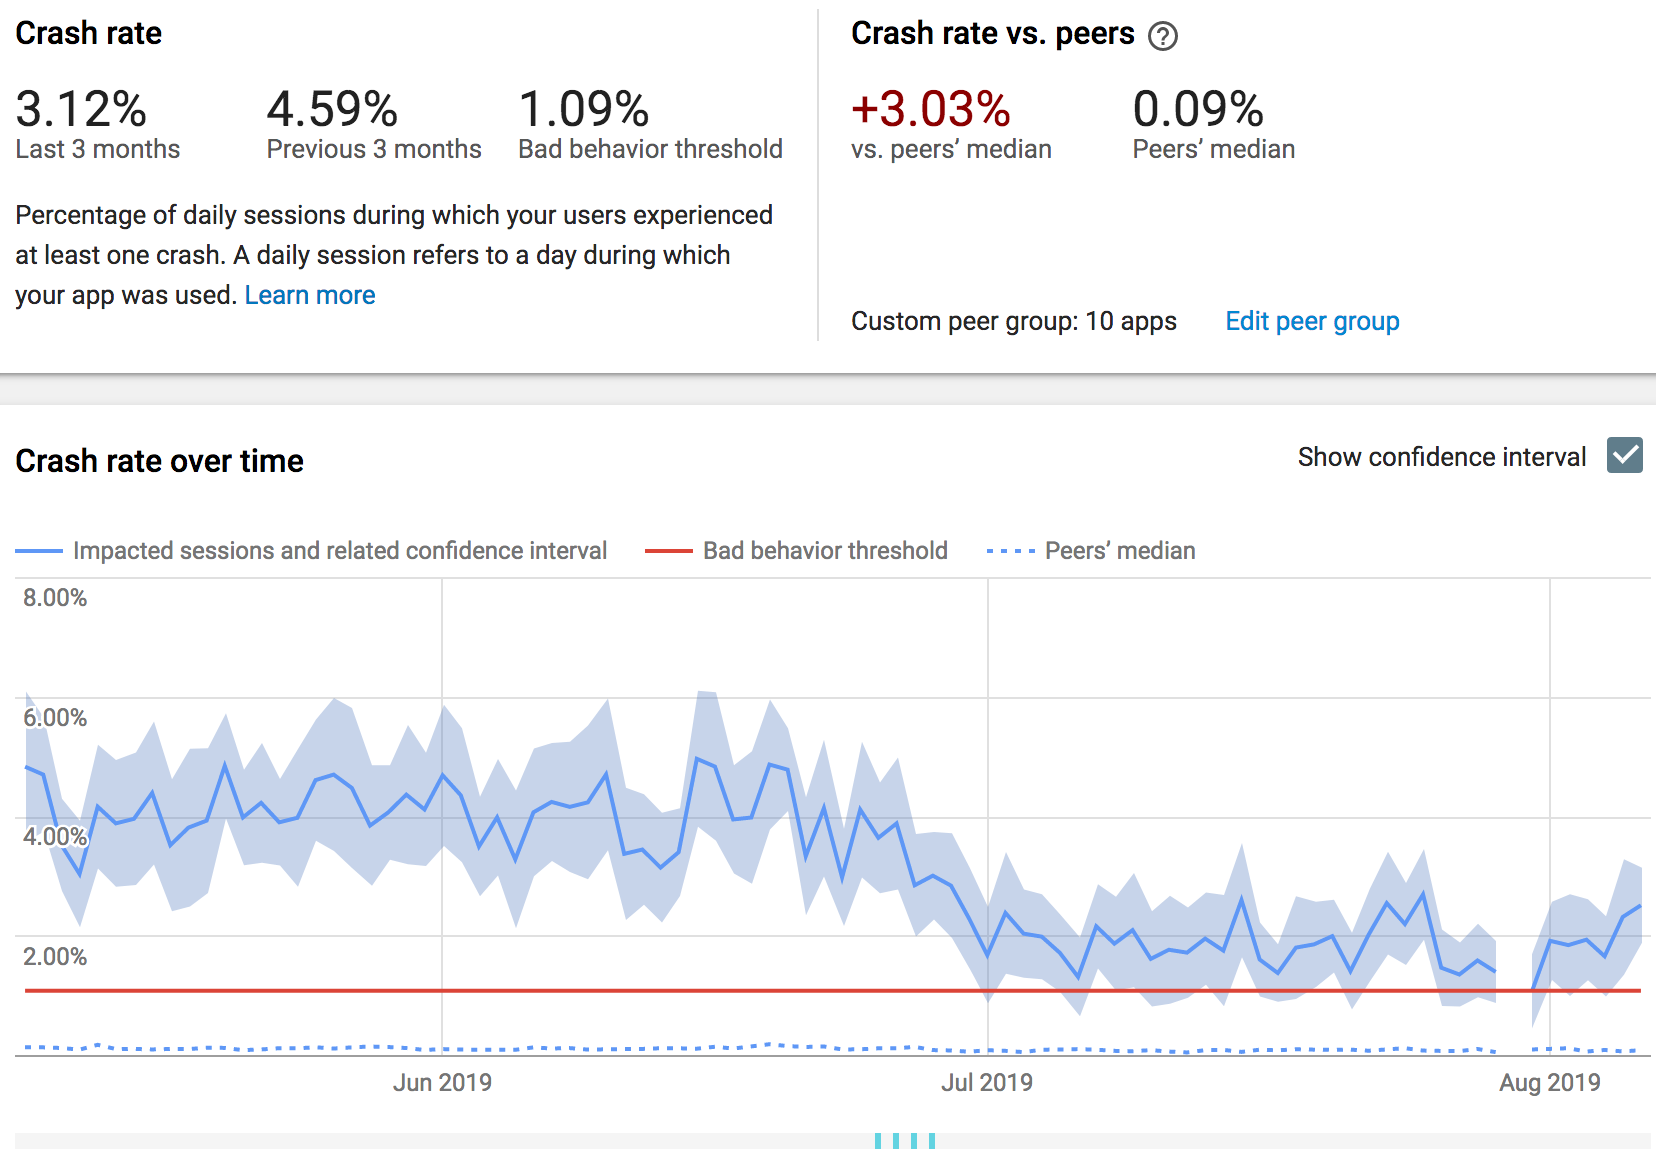
\includegraphics[width=\textwidth]{images/android-vitals-screenshots/kiwix-crash-rate-drops-with-v2_5.png}
    \caption{Kiwix Crash Rate Drops with V2.5 Release}
    \label{fig:kiwix_crash_rate_drops_v2_5}
\end{figure}

\textbf{Phase 2}: Following initial discussions about the crashes being reported in Android Vitals for version 2.5.0 of the Kiwix application, a group of the developers for the Kiwix projects collaborated on a week-long hackathon in Stockholm in August 2019. One of the areas the developers worked on was to focus on identifying and addressing some of the biggest contributors to the high crash rate. 
%
The developers ended up fixing some of the causes of the most frequent crashes with a surprisingly small amount of code of under 25 lines (including 10 lines of text added to the release log)\footnote{\url{https://github.com/kiwix/kiwix-android/pull/1388}}.

MUST-DO provide details of the improvements made after the implementation.


\textbf{Phase 3}: Several developers for the Kiwix project, the lead developer in particular, have been actively reviewing crashes reported by Android Vitals, filing issues, and addressing the causes of the crashes in order to reduce the crash rate and improve the app's stability. Evidence issues that mention crash: 133 closed, 6 open. \footnote{\url{https://github.com/kiwix/kiwix-android/issues?utf8=\%E2\%9C\%93&q=is\%3Aissue+crash}}
%TODO in a longer work, analyse each issue to identify the source of the crash.

Several releases later, each with various changes and improvements aimed at fixing causes of crashes the crash rate was materially lower than when we started, at the time of writing the overall crash rate for the last 7 days is 0.54\% which is inflated because the rash rate for the previous release (3.1.2) spiked at 1.38\%, compared to 0.18\% for release (3.0.5 -  the last production release) and 0.25\% for the recently released fix (3.1.3).


\subsection{Discussion}~\label{case-study-kiwix-discussion}
\textit{(Explore what these outcomes mean for the use of analytics in mobile software more generally).}

\textbf{MUST-DO} explain why statistics and reports aren't available for less popular apps.

\textbf{MUST-DO} describe about the flaws discovered in GPC and Android Vitals and the discussions with Google Engineering.



\subsection{Summary of Kiwix Android Case Study}
% Joe's notes this is not compelling and doesn't compare with the other case studies.
% Why Kiwix, what did I gain, similarities and contrasts, why include in the PhD.

This is a long term study, where I was embedded as part of the development team for a period of the case study. We demonstrated it was practical to use only external, platform, analytics and still able to be effective in reducing the crash rate. For projects that do not use in-app crash reporting the platform tools are sufficient to make material improvements \emph{when the team actively monitors and addresses the crashes reported in the platform level analytics}. The practices need to be applied on a long term basis; with the loss of the project lead who focused on addressing the runtime failures the failure rates are increasing. Entropy increases.

The case study was very useful in terms of providing  control and experiment apps. It was also the first of the experiments that set the scene and the direction for further case-studies.

The analytics reported on both \href{glossary_jvm}{JVM} and native crashes (written in C++) where that code is external and shared with various projects. 

% Provided materials published in various of my papers
This case study also led to the discovery of various flaws in Google Play Console and Android Vitals which led to the meetings, discussions and writing the report for the Google Engineering team. They have improved their product iteratively - v2 still had some flaws v3 has addressed some of these and similarly reduced some of the operability headaches.




%%%%%%%%%%%%%%%%%%%%%%%%%%%%%%%%%%%%%%%%%%%%%%%%%%%%%%%%%%%%%%%%%%%%%%%%
\par\noindent\rule{\textwidth}{0.4pt}
~\textbf{Earlier material follows}






% Following initial discussions about the crashes being reported in Android Vitals for version 2.5.0 of the Kiwix application, we collaborated on a week-long hackathon in Stockholm in August 2019. There, the developers ended up fixing some of the causes of the most frequent crashes with a surprisingly small amount of code of under 25 lines (including 10 lines of text added to the release log)\footnote{\url{https://github.com/kiwix/kiwix-android/pull/1388}}.



\subsection{Examples of real-time crashes}
Each of these examples exemplifies at least one characteristic of the reports that are provided by Android Vitals in Google Play.

\subsubsection{EsxRenderBucket::AddUnbucketedEntries(...)}
This crash is one of the most frequent crashes reported in early October 2020 and has been occurring on an ongoing basis according to Android Vitals for the current release of the Chemistry \& Physics simulations app (release 2020-04). Through analysis of the reports this crash only affects one release of the app (release 5200950) and it does not occur on the other three releases (6200950, 4200950, 3200950). It occurs on multiple manufacturer's device models, and on Android 9.0, 8.1, and 8.0). 

This crash is a native crash and mainly occurs within the context of \texttt{/system/app/Chrome/Chrome.apk} \textit{the web browser app created by Google!} The Kiwix apps rely on an embedded web browser, which is generally Google's Chrome browser, to render (\emph{i.e.} display) the content to the user\footnote{It also appears for other variants of the Android Chrome browser on some devices e.g. \texttt{/data/app/com.android.chrome-bAmCl9DcPfmqf3oKL54Efg==/base.apk (offset 0xbe7000)} and also the Android WebView component~\texttt{/data/app/com.google.android.webview-9ShSu\_81V02zu4ENrAjvJA==/lib/arm/libwebviewchromium.so} (also created by Google).}.

\begin{listing}[H]
\caption{Crash Cluster: EsxRenderBucket::AddUnbucketedEntries} \label{code:crash_cluster_add_unbucketed_entries}
\tiny
\begin{minted}{cpp}
*** *** *** *** *** *** *** *** *** *** *** *** *** *** *** ***
pid: 0, tid: 0 >>> org.kiwix.kiwixcustomphet <<<

backtrace:
  #00  pc 00000000001535a0  /vendor/lib/egl/libGLESv2_adreno.so (EsxRenderBucket::AddUnbucketedEntries(EsxCmdBufType, unsigned int)+132)
  #01  pc 0000000000152b17  /vendor/lib/egl/libGLESv2_adreno.so (EsxRenderBucket::BucketRenderingCmds(EsxRenderBucketParams*)+740)
  #02  pc 0000000000186a6d  /vendor/lib/egl/libGLESv2_adreno.so (EsxContext::BucketRenderingCmds(int)+712)
  #03  pc 00000000000e6987  /vendor/lib/egl/libGLESv2_adreno.so (EsxContext::BindDrawFramebuffer(EsxFramebufferObject*)+178)
  #04  pc 00000000000b6a5d  /vendor/lib/egl/libGLESv2_adreno.so (EsxContext::GlBindFramebuffer(unsigned int, unsigned int)+332)
  #05  pc 0000000001b8c659  /system/app/Chrome/Chrome.apk (offset 0x80c000)
\end{minted}

\end{listing}

Of the 53 crash clusters reported over the last 60 days for all Android versions and version 5200950 of the app, installed from Google Play, 16 of the 53 crash clusters are for this crash.

Searching local logs, generated using the opensource software~\texttt{vitals-scraper} that we created as part of this research we can see the same crash cluster has occurred in some, not all, of the Kiwix applications. The command used to find the files that contain this crash cluster is:~\texttt{grep -c EsxRenderBucket::AddUnbucketedEntries * | sort -t ':' -k 2 -g}. This returns a list of the files, sorted by the number of matches for the string found in each of the files. Here are the entries with at least one match.

\begin{listing}[H]
\caption{Logs that include crash cluster: EsxRenderBucket::AddUnbucketedEntries} \label{code:vitals_scraper_logs_add_unbucketed_entries}
\footnotesize
\begin{minted}{text}

android-crash-clusters-org.kiwix.kiwixcustomphet_1572958874833.json:2
android-crash-clusters-org.kiwix.kiwixmobile_1599898794048.json:2
phet-1-day-android-crash-clusters_1569599996989.json:2
android-crash-clusters-org.kiwix.kiwixcustomphet_1572966654935.json:3
android-crash-clusters-org.kiwix.kiwixmobile_1577913956806.json:3
android-crash-clusters-org.kiwix.kiwixcustomphet_1574380641173.json:4
android-crash-clusters-org.kiwix.kiwixcustomphet_1572976000060.json:5
android-crash-clusters-org.kiwix.kiwixcustomphet_1577913523667.json:5
android-crash-clusters-org.kiwix.kiwixcustomphet_1601883786819.json:5
wikimed-60-days-android-crash-clusters_1568705009571.json:6
phet-7-days-android-crash-clusters_1569484818005.json:13
android-crash-clusters-org.kiwix.kiwixcustomphet_1573403158401.json:14
android-crash-clusters-org.kiwix.kiwixcustomphet_1599898464809.json:14
phet-60-days-android-crash-clusters_1568703927627.json:18
android-crash-clusters-org.kiwix.kiwixcustomphet_1572903426940.json:21
phet-60-days-android-crash-clusters_1565933377493.json:21
android-crash-clusters-org.kiwix.kiwixcustomphet_1572812538185.json:25
\end{minted}

\end{listing}

From these results the crash occurs most often in the Physics \& Chemistry simulation custom app (these include the phrase `phet'\footnote{`phet' is the term used for the source of the contents used in this custom app, i.e. the source of the various Chemistry and Physics simulations, written in HTML5. They are extremely rich in terms of their content and dynamic rendering as they provide interactive, dynamic simulations.} as part of the filename. It also occurred relatively infrequently in two other of the apps: five times in the core Kiwix app, and six times in the Wikipedia in English app. The core Kiwix app can be used with the same contents as the project bundles in the custom apps, so some of the crashes~\emph{might} be for the same content, we don't know enough from the stack trace to determine the contents. the reasons for the error in the custom WikiMed app are not known at this stage. 

Searching online, using Google Search, for \texttt{EsxRenderBucket::AddUnbucketedEntries} finds a similar stack trace occurs with the Unity SDK and it appears to be related to a particular chipset:
\begin{itemize}
    \item \href{https://developer.qualcomm.com/forum/qdn-forums/software/adreno-gpu-sdk/67924}{Forums - Help with crash in {\footnotesize libGLESv2\_adreno.so (EsxRenderBucket::AddUnbucketedEntries)}} 2020
    % \item \href{https://github.com/flutter/flutter/issues/38676}{/system/vendor/lib/egl/libGLESv2_adreno.so #38676} 2019
    % \item \href{https://stackoverflow.com/questions/29728931/libglesv2-adreno-so-game-crash-in-galaxy-note-4-and-lollipop-5-0}{libGLESv2_adreno.so game crash in Galaxy Note 4 and Lollipop 5.0} 2015
    \item \href{https://forum.unity.com/threads/unity-2019-android-build-crashes-on-devices-using-adreno-506-gpu.712229/}{Unity 2019 Android build crashes on devices using Adreno 506 GPU}. This bug report includes several different method names where the crash occurs. Various developers report the issue, \href{https://forum.unity.com/members/waldgeist.1371619/}{Waldgeist} reporting the one with this method name.
\end{itemize}

The bug appears hard for developers to reproduce and from the app developer's perspective it happens in software they cannot fix themselves. 

As Ogien reports in~\href{https://forum.unity.com/threads/unity-2017-2-crashes-vs-5-6-2f1.511995/}{Unity 2017.2 Crashes vs 5.6.2f1} they may be able to identify correlations (in this example using a screenshot from Android Vitals, I believe, as shown in Figure~\ref{fig:unity-2017-2-android-vitals-annotated-graph}). The Unity support team state the bug may have been fixed and the developer promised to try the new release and report back at the time, in 2018, however they have not done so online at least\footnote{This user was online more recently, including \nth{24} September 2020.} so that issue has an indeterminate result from a research perspective.

\begin{figure}[htbp!]
    \centering
    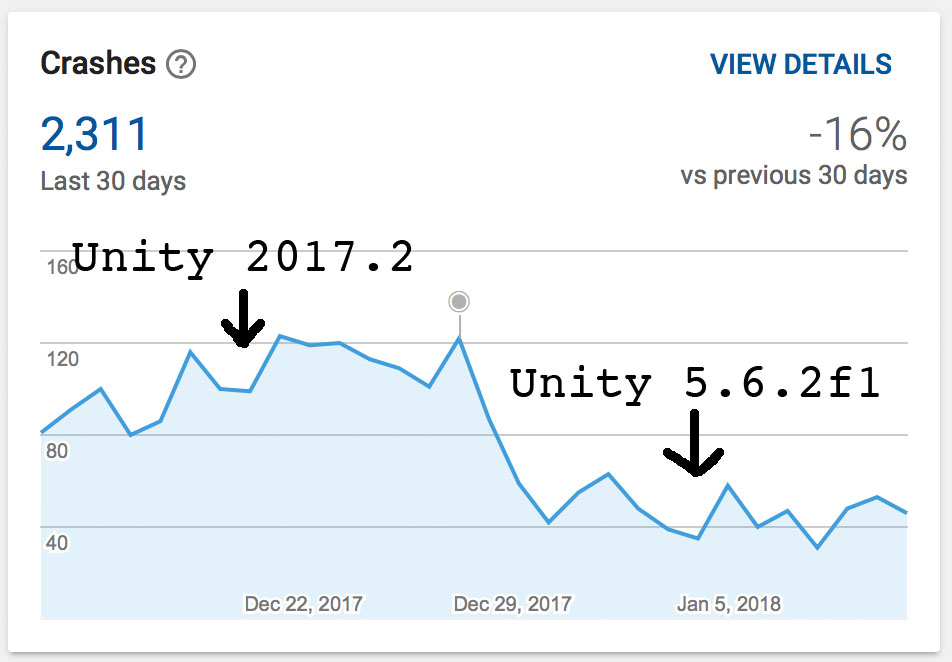
\includegraphics[width=12cm]{images/unity-forum/unity-2017-2-android-vitals.jpg}
    \caption{Unity 2017.2 Android-Vitals annotated graph (\url{https://forum.unity.com/threads/unity-2017-2-crashes-vs-5-6-2f1.511995/}}
    \label{fig:unity-2017-2-android-vitals-annotated-graph}
\end{figure}

MUST-DO Discuss the augmented crash stack trace utility, how it works, and why we did~\emph{not} use it in Google Play apps.


\subsection{Lessons learned from this case study}

As~\citep{kidwell2015_toward_fault_taxonomy_application_of_software_analytics} notes, previous research by~\citep{weider1998_software_fault_prevention_in_coding_and_RCA} nearly half the faults were introduced during coding and \emph{``...many of the faults were preventable"}. These results were borne out in the Kiwix Android case study where some of the most frequent crashes were null pointer errors in the Java code. For the Kiwix Android project one of the longer term challenges was the youth of many of the volunteer contributors including some of the development leads who were often teenagers and pre-undergraduate level software developers who wouldn't have the expertise expected of professional software developers\footnote{(They often joined via Google Code-in~\citep{google_code_in_archive} or Google Summer of Code~\citep{google_summer_of_code}).}. While there may well be training techniques and software tools, including Android Lint, that may have been able to find some of the causes of the crashes reported by Android Vitals it's unlikely that these volunteers would choose to use those tools or want to undergo training. And as interviews with developers demonstrated the perceived effort of dealing with static analysis reports and the volume of false positives mean developers don't use static analysis tools very often to find bugs~\citep{johnson2013_why_dont_devs_use_static_analysis}.

\subsection{Summary of Kiwix Android Case Study}
TBC